
%%%%%%%%%%%%%%%%%%%%%%% file typeinst.tex %%%%%%%%%%%%%%%%%%%%%%%%%
%
% This is the LaTeX source for the instructions to authors using
% the LaTeX document class 'llncs.cls' for contributions to
% the Lecture Notes in Computer Sciences series.
% http://www.springer.com/lncs       Springer Heidelberg 2006/05/04
%
% It may be used as a template for your own input - copy it
% to a new file with a new name and use it as the basis
% for your article.
%
% NB: the document class 'llncs' has its own and detailed documentation, see
% ftp://ftp.springer.de/data/pubftp/pub/tex/latex/llncs/latex2e/llncsdoc.pdf
%
%%%%%%%%%%%%%%%%%%%%%%%%%%%%%%%%%%%%%%%%%%%%%%%%%%%%%%%%%%%%%%%%%%%


\documentclass[runningheads,a4paper]{llncs}

\usepackage{amssymb}
\setcounter{tocdepth}{3}
\usepackage{graphicx}
\usepackage{algorithm}
\usepackage[noend]{algpseudocode}
\usepackage{float}

\usepackage{url}
\urldef{\mailsa}\path|{sorina.maciuca,gil.mcvean, zamin.iqbal}@well.ox.ac.uk| 
\urldef{\mailsb}\path|{carlos.delojoelias}@ndm.ox.ac.uk| 

\newcommand{\keywords}[1]{\par\addvspace\baselineskip
\noindent\keywordname\enspace\ignorespaces#1}

\begin{document}

\mainmatter  % start of an individual contribution

% first the title is needed
\title{A natural encoding of genetic variation in a Burrows-Wheeler Transform  to enable mapping and genome inference}

% a short form should be given in case it is too long for the running head
\titlerunning{Encoding genetic variation in a BWT}

% the name(s) of the author(s) follow(s) next
%
% NB: Chinese authors should write their first names(s) in front of
% their surnames. This ensures that the names appear correctly in
% the running heads and the author index.
%
\author{Sorina Maciuca%
\and Carlos delOjo Elias\and Gil McVean \and Zamin Iqbal}
%
\authorrunning{Encoding genetic variation in a BWT}
% (feature abused for this document to repeat the title also on left hand pages)

% the affiliations are given next; don't give your e-mail address
% unless you accept that it will be published
\institute{Wellcome Trust Centre for Human Genetics,\\
University of Oxford, Roosevelt Drive, Oxford OX3 7BN, UK\\
\mailsa\\
\mailsb\\
}


\toctitle{Lecture Notes in Computer Science}
\tocauthor{Authors' Instructions}
\maketitle


\begin{abstract}
We show how positional markers can be used to encode genetic variation within a Burrows Wheeler Transform (BWT), and use this to construct a generalisation of the traditional ``reference genome", incorporating known variation within a species. Our goal is to support the inference of the closest mosaic of previously known sequence to the genome(s) under analysis.\\ Our scheme results in an increased alphabet size, and by using a wavelet tree encoding of the BWT we reduce the performance impact on rank operations. We give a specialised form of the backward search that allows variation-aware exact matching. We implement this, and demonstrate the cost of constructing an index of the whole human genome with 80 million genetic variants is 31GB of RAM,  below that of previous implementations. We also show that inferring a closer reference can close large kilobase-scale holes in mapping pileups in \textit{P. falciparum}
\keywords{pan-genome, Burrows-Wheeler Transform, FM index, genome}
\end{abstract}

\section{Introduction}

Genome sequencing involves breaking  DNA into fragments, identifying substrings (called "reads") and then inferring properties of the genome. Recently, it has become possible to study within-species genetic variation on a large scale \cite{1000g,arabi,pombe}, where the dominant approach is to match substrings to the canonical "reference genome" which is constructed from an arbitrary individual.  This problem (``mapping") has been heavily studied  (see \cite{reinert}) and the Burrows Wheeler Transform \cite{bwt} underlies the two dominant mappers - bwa \cite{bwa} and bowtie \cite{bowtie}. Mapping reads to a reference genome is a very effective means of detecting genetic variation involving single character changes (SNPs - single nucleotide polymorphisms). However this method becomes less effective the further the genome differs from the reference.  Many important regions of genomes are highly diverse, and so sequence reads from a random genome can very easily fail to map to the reference. 

We  want to build a representation of the genome of a species which incorporates N genomes and supports the following inference. We take as input, sequence data from a new sample of our species, and  an estimate of how many genomes the sample contains and their relative proportions - e.g. a normal human sample would contain 2 genomes in a 1:1 ratio, a bacterial isolate would contain 1 genome, and a malaria sample might contain 3 genomes in the ratio 10:3:1. We would then infer the sequence of the underlying genomes. In this paper we describe a method for encoding genetic variation designed to enable this approach. 

Genomes evolve (broadly speaking) by two processes - mutation (changing a single character, or less frequently, inserting or deleting a few) and recombination (either two chromosomes exchange a chunk of DNA, or one chromosome copies a chunk from another). Thus once we have seen many genomes of a given species, a new genome is likely to look like a mosaic of genomes we have seen before.  If we can infer a close mosaic, we have found a ``personalised reference genome", and reads are more likely to exact-match. This approach was first described in \cite{dilthey}, applied to to the human MHC region. However their implementation was quite specific to the region and would not scale to the whole genome. Valenzuela et al \cite{valen} have recently also espoused a find-the-closest-reference approach.

Other ``reference graph" approaches have been published \cite{korbinian,siren1,huang}, generally approaching just the alignment step.  Siren \textit{et al} developed an  method (GCSA \cite{siren1}) - however construction costs for a whole human genome plus a set of SNPs required more than 1 Tb of RAM. Huang et al \cite{huang} developed an FM index encoding of a reference genome-plus-variation (``bwbble") by extending the genetic alphabet to encode single-character variants with new characters and then concatenating padded indel variants to the end of the reference genome. Bwbble allows reads to align smoothly across multiple SNPs and up to one indel. We do something similar, but treat all variation in an equivalent manner.  While completing this paper, the preprint for GCSA2 was published (\cite{siren2}), which drops RAM usage of human genome index construction to $<$100GB at the cost of $>$1Tb of disk I/O.   

 We show below how to encode a set of genomes, or a reference plus  genetic variation, in an FM index which naturally distinguishes alternate alleles (defined below). We extend the well known  BWT backward search, and show how read-mapping can be performed in a way that allows reads to cross multiple variants, allowing recombination to occur naturally. Our data structure  supports bidirectional search (which underlies the Super Maximal Exact Match algorithms of bwa-mem \cite{bwa}), but currently we have only implemented exact matching. We show that index construction is relatively cheap, encoding the human genome and 8.3 million genetic variants from the 1000 genomes project using just 36 GB of RAM on a single core in 7 hours. We go on to show how inferring a personalised reference results in better genome inference, looking at a highly challenging region - the MSP3.4 gene of \textit{P. falciparum} where alleles differ by one SNP every 3 bp.  


\section{Background: Compressed Text Indexes}

\subsubsection{Burrows-Wheeler Transform.}
The Burrows-Wheeler Transform (BWT) of a string is a reversible permutation of its characters that was originally developed for compression \cite{bwt}.The BWT of a string $T=t_1t_2 \ldots t_n$ is constructed by sorting its $n$ cyclic shifts $t_1t_2 \ldots t_n$, $t_2 \ldots t_n t_1$, \ldots,  $t_n t_1 \ldots t_{n-1}$ in lexicographic order. The matrix obtained is called the Burrows-Wheeler Matrix (BWM) and the sequence from its last column is the BWT. Storing the first and last column of the BWM is sufficient for finding the number of exact matches of a query in $T$. For locating the position of the matches in $T$ an additional data structure is required, the suffix array. 

\subsubsection{Suffix Arrays.} The suffix array of a string $T$ is an array of integers that provides the starting position of $T$'s suffixes, after they have been ordered lexicographically. Formally, if $T_{i,j}$ is the substring $t_i t_{i+1} \ldots t_j$ of $T$ and SA is the suffix array of $T$, then $T_{SA[1],n}<T_{SA[2],n}<\ldots <T_{SA[n],n}$. It is related to the BWT, since looking at the substrings preceding the terminating character $\$$ in the BWM rows gives the suffixes of $T$ in lexicographical order. 
\subsubsection{Backward search}
Any occurrence of a pattern $P$ in text is a prefix for some suffix of $T$, so all occurrences will be adjacent in the suffix array of $T$, since suffixes starting with $P$ are sorted together in a SA-interval. Let $C[a]$ be the total number of occurrences in $T$ of characters smaller than $a$ in the alphabet. Then if $P'$ is a suffix of the query $P$ and $[l(P'),r(P')]$ is its corresponding SA-interval, then the search can be extended to $aP'$ by calculating the new SA-interval:
\newline
\begin{equation} 
l(aP')=C[a]+rank_{a}(BWT,l(P')-1)+1 
\end{equation} 

\begin{equation} 
r(aP')=C[a]+rank_{a}(BWT,r(P)),
\end{equation}

where the operation $rank_a(S,i)$ returns the number of occurences of symbol $a$ in $S[0,i]$. The search starts with the SA-interval of the empty string, $[1,n]$ and successively adds one character of $P$ in backward order. When the search is completed, it returns a SA-interval $[l,r]$ for the entire query $P$. If $r \geq l$, there are $r-l+1$ matches for $P$ and their locations in $T$ are given by $SA[i]$ for $l \leq i \leq r$. Otherwise, the pattern does not exist in $T$. If the $C$-array and the ranks have already been stored, the backward search can be performed in $O(|P|)$ time in strings with DNA alphabet.

\subsubsection{Wavelet Trees}
Rank queries scale linearly with the alphabet size by default. The wavelet tree is a data structure designed to store strings with large alphabets efficiently and provide rank calculations in logarithmic time. A wavelet tree converts a string into a balanced binary-tree of bitvectors, whose root is built by taking the sorted alphabet and replacing the lower half of smaller symbols with a 0, and the other half of larger symbols with a 1 in the string. This creates ambiguity initially, but at each tree level, each half of the parent node's alphabet is re-split into 2 and re-encoded, so the ambiguity lessens as the tree is traversed in depth. At the leaves, there is no ambiguity at all. The tree is defined recursively: take the lexicographically ordered alphabet, split it into 2 equal halves; in the string corresponding to the current node (start with original string at root), replace the first half of letters with 0 and the other half with 1; the left child node will contain the 0-encoded symbols and the right child node will contain the 1-encoded symbols, preserving their order from the original string; reapply the first step for each child node recursively until the alphabet left in each node contains only one or two symbols (so a 0 or 1 determines which symbol it is).

 \begin{figure}
\centering
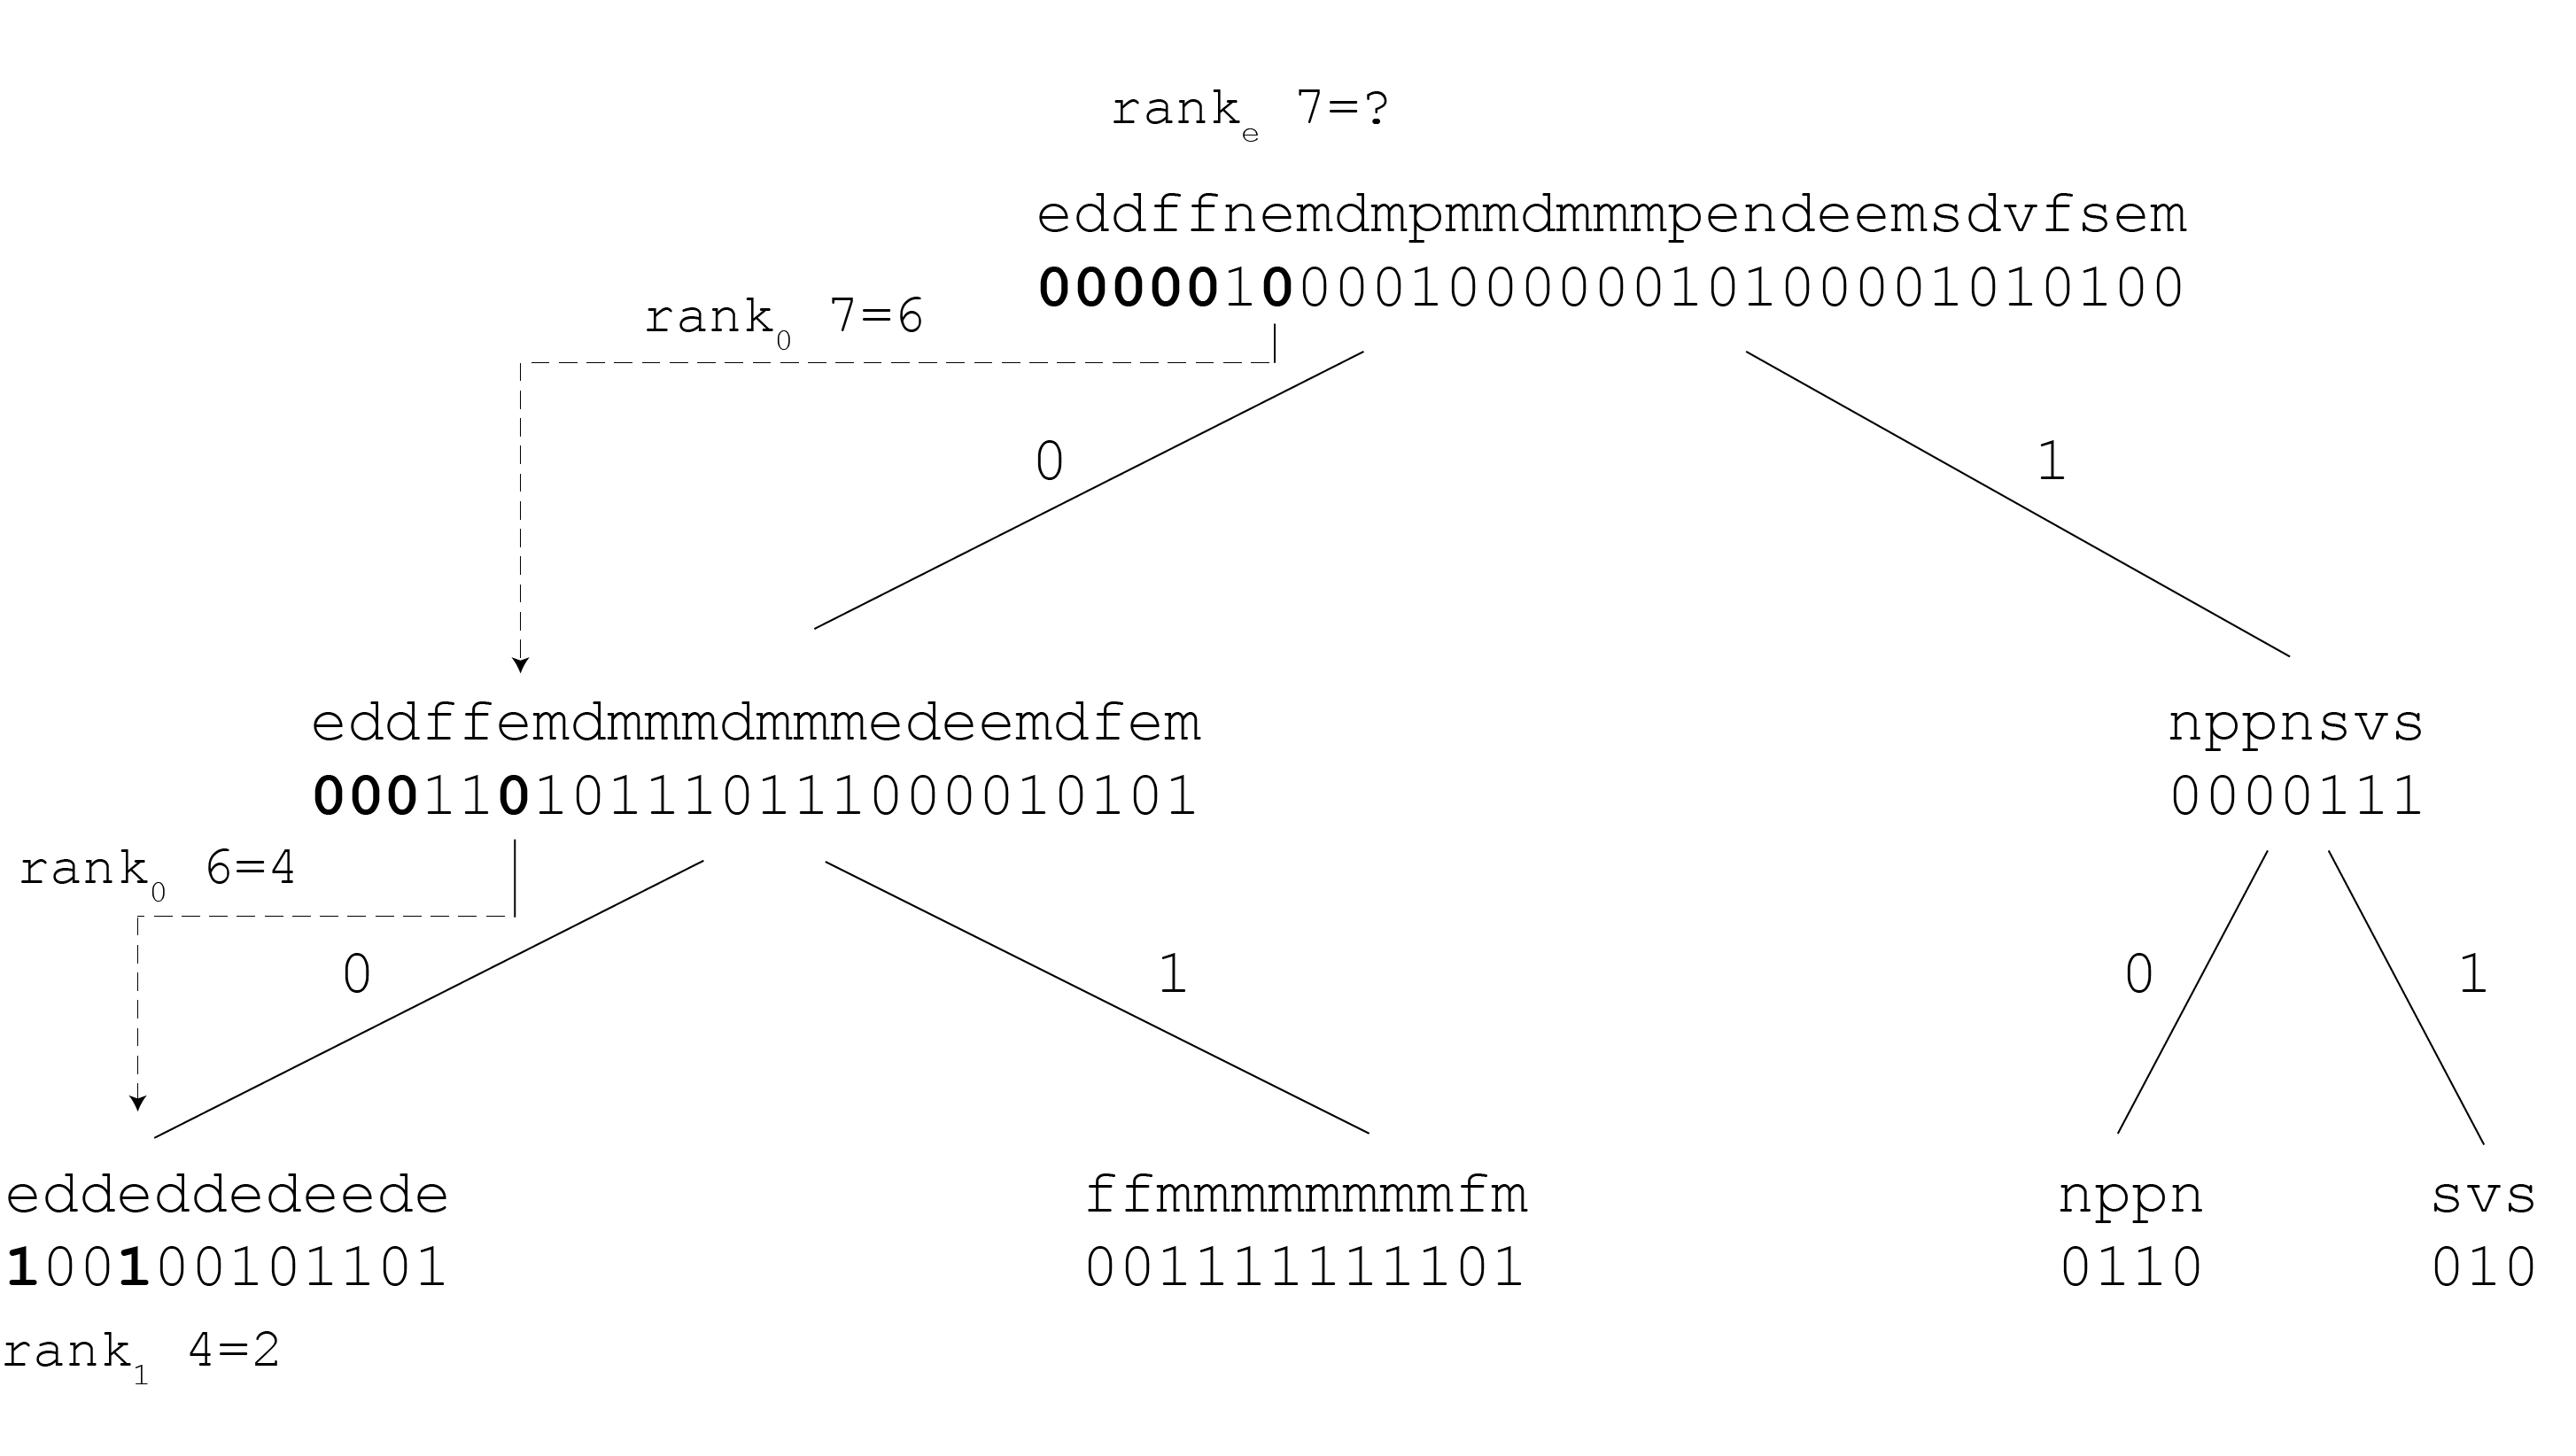
\includegraphics[height=6cm]{wavelet_tree.png}
\caption{Wavelet tree encoding of a string; we return to this string in Figure 2 below, as an encoding of a PRG. Calculating the rank of the marked C is performed by repeated rank() calls moving down the binary tree until the alphabet remaining is just 2 characters.}
\label{fig:wt}
\end{figure}

In order to answer a rank query over the original string with large alphabet, repeated rank queries over the bitvectors in the wavelet tree nodes are used as a guide to the  subtree that contains the leaf where the queried symbol is non-ambiguously encoded. The rank of the queried symbol in this leaf is equal to its rank in the original string. The number of rank queries needed to reach the leaf is equal to the height of the tree, i.e. $\log_{2} {|\Sigma|}$ if we let $\Sigma$ be the set of symbols in the alphabet. Computing ranks over binary vectors can be done in constant time, so a rank query in a wavelet tree-encoded string has complexity $O(\log_{2} {|\Sigma|})$. 

\section{Encoding a variation-aware reference structure}

\subsection{Terminology}
A \textit{variant site} or \textit{site} is a region of the chromosome where there are a number of alternative options for what sequence can be present.
These alternatives are termed \textit{alleles} and might be as short as a single character, or could be many hundreds of characters long. A  \textit{pan-genome} means a representation of a number (greater than 1) of genomes within a species. 

\subsection{PRG Encoding}



Following \cite{dilthey}, we use a linear PRG conceptually equivalent to a directed, acyclic, partial order graph, that is generated from a reference sequence and a set of alternative sequences at given variation sites. The graph is linearised into a long string over an alphabet extended with new symbols marking the variants, for which the FM-index can be constructed. 


\begin{figure}
\centering
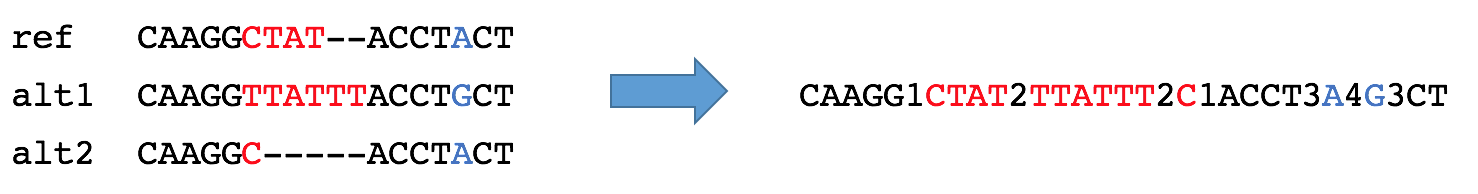
\includegraphics[height=1.5cm]{linPRG}
\caption{A simple PRG linearised according to our encoding. The first site has 3 alleles, which do not here look at all similar, and the second is a SNP. The wavelet tree shown in the previous section is built on this example, and subsequent figures will make further use of it.}
\label{lab}
\end{figure}



Building this data structure requires multiple steps. 
\begin{enumerate}
\item First, corresponding regions of shared (exact match) sequence between the input  genomes must be identified. These must be of size $k$ at least (where $k$ is pre-defined), and  act as anchors for the coordinates of the variation sites. 
\item Second, for any site between two anchor regions, the set of possible haplotypes must be determined from the input genomes, but  do not need to be aligned. Indels are naturally supported by haplotypes of different lengths.
\item Each variation site is assigned two unique numeric identifiers, one even and one odd, and will be called variation markers. The odd identifiers will mark variation site boundaries and will sometimes be referred to as site markers. The even identifiers will mark alternative allele boundaries and will sometimes be referred to as allele boundary markers.
\item For each variation site, its left anchor is added to the linear PRG, followed by its odd identifier. Then each sequence coming from that site, starting with the reference sequence, is successively added to the linear PRG, followed by the even site identifier, except the last sequence, which is followed by the odd identifier.
\item Convert the linear PRG to integer alphabet ($A\rightarrow 1$, $C\rightarrow2$, $G\rightarrow3$, $T\rightarrow4$, variation site identifiers $\rightarrow$ 5,6,...)
\item The FM-index (suffix array, BWT, wavelet tree over BWT) of the linear PRG is constructed and we will call this the vBWT.
\end{enumerate}

An illustration of these steps on a toy example is given in Figure 2.


Importantly, \textit{the markers force the ends of alternative sequences coming from the same site to be sorted together in a separate block in the Burrows-Wheeler matrix, even if they do not have high sequence similarity}. Therefore, alternative alleles from each site can be queried concurrently.


\subsection{Graph structure: constraints}


We show in Figure 3a two chromosomes which differ by 3 SNPs, and in 3b) and 3c) give two graph encodings. Both represent the sequence content equally well, and we allow both.
 However, we show in 3d) an example where a long deletion lies ``over" two other alleles. We would encode this in our PRG as shown in 3e). This works, but results in many alternate alleles. An alternative would be to allow ``nested" variation, where variants lie on top of other alleles, as shown in Figure 3f). This could certainly be encoded in our system, but we do not allow it for our initial implementation, as it would potentially impact mapping speed. Note that this constraint is shared by bwbble.

\begin{figure}
\centering
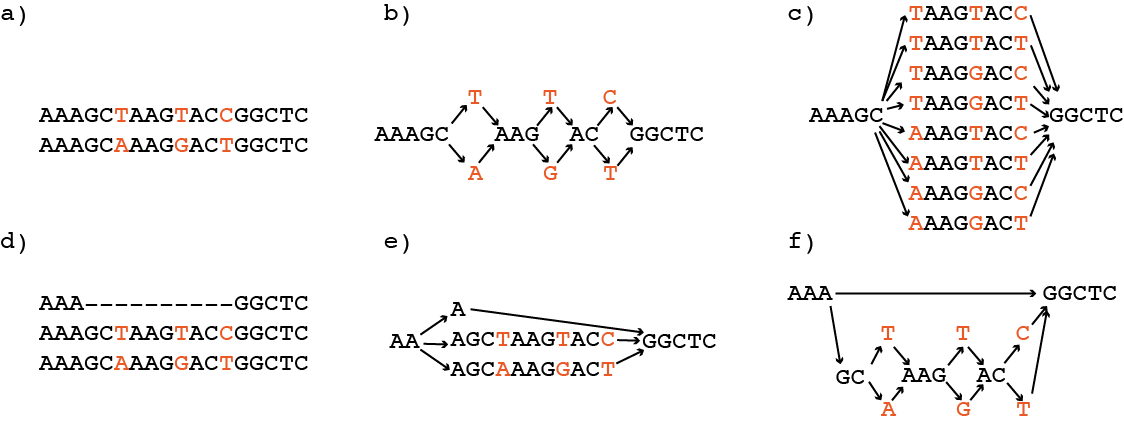
\includegraphics[height=4.5cm]{graph_construction.png}
\caption{PRG graph structure. The sequences shown in Figure 3a) could be represented either as 3 separate mutations (shown in b)),or enumerated as 8 small haplotypes , shown in c). Both are supported by our encoding. Similarly, the sequences in d) could be represented in our implementation as shown in e). However, we do not support ``nesting" of alleles, as shown in f).}
\label{lab}
\end{figure}






\section{Variation aware backward search in vBWT}

In this section, we present a modified backward search algorithm for exact matching against the vBWT that is aware of alternative sequence paths. When reads align to the non-variable part of the linear PRG or when a variant locus is long enough to enclose the entire read, the usual backward search algorithm can be used. Otherwise, when the read must cross variation site junctions in order to align, site identifiers and some alternative alleles must be ignored by the search. This means a read can align to multiple substrings of the linear PRG that may not be adjacent in the BWM, so the search can return multiple SA-intervals. We give pseudocode in Algorithm 1 below, and outline the idea in Figure 4.




\begin{figure}
\centering
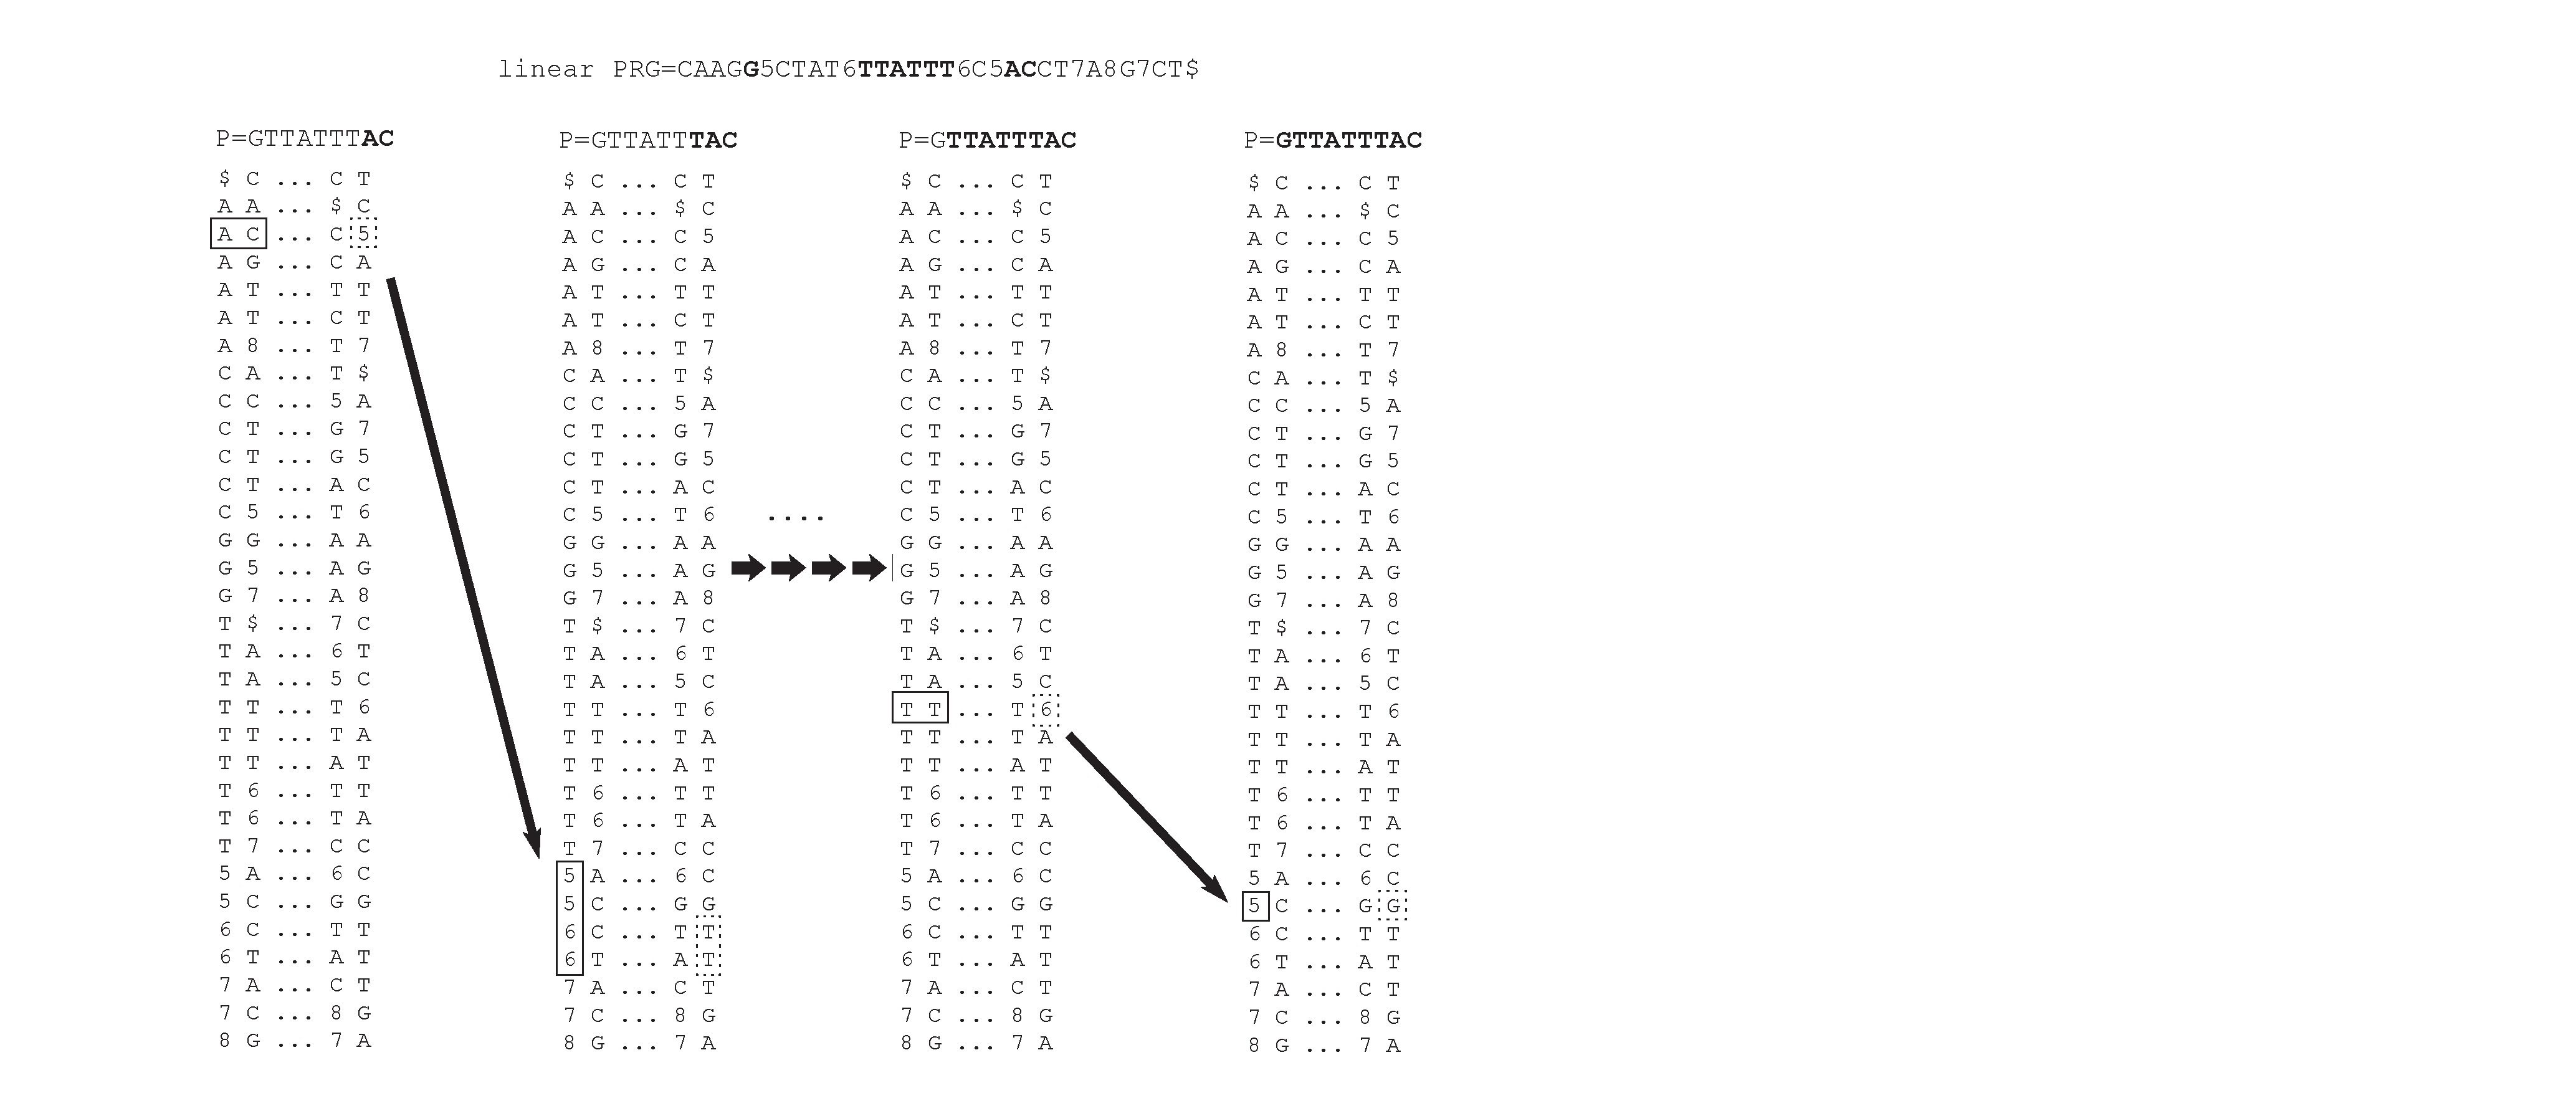
\includegraphics[height=7cm]{BWT.pdf}
\caption{Backward search across vBWT.  We start at the right-hand end of the read GTTATTTAC, with the character C, and as we extend we hit the character 5, signalling the start or end of a variation locus. We check with a mask, and find it is the end. Therefore the read must now continue into one of the alleles, signalled by the number 6. Continuing in this manner (the shorter arrows signify multiple intermediate steps not shown) we are able to align across the site.}
\label{fig:example}
\end{figure}

At each step in backward search, before extending to the next character, we need to check whether the current matched read substring is preceded by a variation marker anywhere in the linear PRG. A scan for symbols larger than 4 (``range\_search\_2d" in the pseudocode) must be performed in the BWT within the range given by the current SA-interval. If a variation marker is found and it is an odd number, the read is about cross a site boundary, i.e. is about to walk in or walk out of a site. The suffix array can be queried to find the position of the two odd numbers in the linear PRG: the number occurring at a smaller position will mark the beginning of site and the other one will mark the end of site.  

\begin{algorithm}[H]
\caption{Modified backward search} \label{bsearch}
\textbf{Input:} \textrm{pattern} $P[0,m]$ \textrm{and FM-index of PRG in integer alphabet}\\
\textbf{Output:} \textrm{list of SA intervals corresponding to matches of P} 
\begin{algorithmic}[1]
\State $l \gets C(P[m])$
\State $r \gets C(P[m]+1)$
\State $i \gets m-1$
\State $\texttt{SA\char`_int}={[l,r)}$
\State $\texttt{Extra\char`_int}=\emptyset$   \Comment keep list of SA intervals
\While {$i > 0$ and $\texttt{SA\char`_int} \neq \emptyset$}
\ForAll {$[l,r) \in \texttt{SA\char`_int}$} 
\State $M \gets \texttt{WT.range\char`_search\char`_2d} (l,r-1,5,|\Sigma|)$ \Comment find variation site markers
\ForAll {$(idx,num) \in M$}  \Comment $ idx\in [l,r), num\in[5,\Sigma]$
\If {$num\%2=0$}
\State $\texttt{odd\char`_num}=num-1$
\Else
\State $\texttt{odd\char`_num}=num$
\EndIf
\If {$CSA[C(\texttt{odd\char`_num})]<CSA[C(\texttt{odd\char`_num})+1]$}
\State $\texttt{start\char`_site} \gets C(\texttt{odd\char`_num})$, $\texttt{end\char`_site} \gets C(\texttt{odd\char`_num})+1$
\Else 
\State $\texttt{start\char`_site} \gets C(\texttt{odd\char`_num})+1$, $\texttt{end\char`_site} \gets C(\texttt{odd\char`_num})$
\EndIf
\If {$num \%2=1$ and $CSA[idx]=CSA[\texttt{site\char`_end}]+1$}
\State $\texttt{Extra\char`_int}=\texttt{Extra\char`_int} \cup \{[C(num),C(num+2))\}$
\Else
\State $\texttt{Extra\char`_int}=\texttt{Extra\char`_int} \cup \{[C[\texttt{start\char`_site}], C[\texttt{start\char`_site}]+1)\}$
\EndIf
\EndFor
\EndFor
\State $i \gets i-1$
\State $\texttt{SA\char`_int}=\texttt{SA\char`_int} \cup \texttt{Extra\char`_int}$
\ForAll {$[l,r) \in \texttt{SA\char`_int}$} 
\State $l=C(P[i])+rank_{BWT}(P[i],l-1)$
\State $r=C(P[i])+rank_{BWT}(P[i],r)$
\EndFor
\EndWhile
\end {algorithmic}
\end{algorithm}


If the search cursor is next to the start of the site, it is just the site marker that needs to be skipped so the SA-interval (size 1) of the suffix starting with that marker needs to be added to the set of intervals that will be extended with the next character in the read. If the search cursor is next to the end of a site, all alternative alleles from that site need to be queried. Their ends are sorted together in the BWM because of the markers, so they can be queried concurrently by adding the SA-interval of suffixes starting with all numbers marking that site (even and odd). 


If the variation marker found is an even number, the read is about to cross an allele boundary, which means its current suffix matches the beginning of an alternative allele and the read is about to walk out of a site, so the search cursor needs to jump to the start of site. As previously described, the odd markers corresponding to that site can be found in the sorted first column of the BWM, and then querying the suffix array decides which one marks the start of site. Then the SA-interval (size 1) for the BWM row starting with this odd marker is recorded.
Once the check for variation markers is finished and all candidate SA-intervals have been added, each interval can be extended with the next character in the read by using equations 1 and 2.




\section{Performance}
\subsection{Construction cost : the human genome}
We   constructed a PRG from the human reference genome (GRC37 without ``alt" contigs) plus the 1000 genomes final VCF (12GB in size) \cite{1000g}, as described below. We first  excluded structural variants which did not have precisely specified alleles, and variants with allele frequency below 5\% (rare variation offers no benefit as use the PRG to find a mosaic reference which differs ideally by isolated SNPs only). If two variants occurred at consecutive bases, they were merged into one, and all possible haplotypes enumerated. If the VCF contained two consecutive records which overlapped, the second was discarded. This resulted in a dataset of 7.4 million SNPs and 978000 indels. We give construction costs in Table 1, along with comparative figures for Bwbble with identical input. 
 
\begin{table}
\caption{FM index construction costs for human reference genome plus 1000 genomes variants}
\centering
\begin{tabular}{c c c}
\hline
Software  & Memory(GB) & Time (hrs/mins)\\
\hline
vBWT  & 36  & 7h5m \\
Bwbble  & 60 &  1h5m \\ 
\hline
\end{tabular}
\end{table}

For comparison, using common Finnish SNPs, GCSA took over 1TB of RAM building chromosomes separately and pruning the graph in high diversity regions. GCSA2 reduces the memory footprint to below 128GB RAM, running in 13 hours with 32 cores, and using  over 1Tb of I/O to fast  disk.  Our vBWT construction has a lower  memory cost than GCSA, GCSA2 and bwbble,  is faster than GCSA/GCSA2, has no (significant) I/O burden, but is significantly slower than bwbble. 



\subsection{Inferring a Closer Reference Genome}

\begin{figure}
\centering
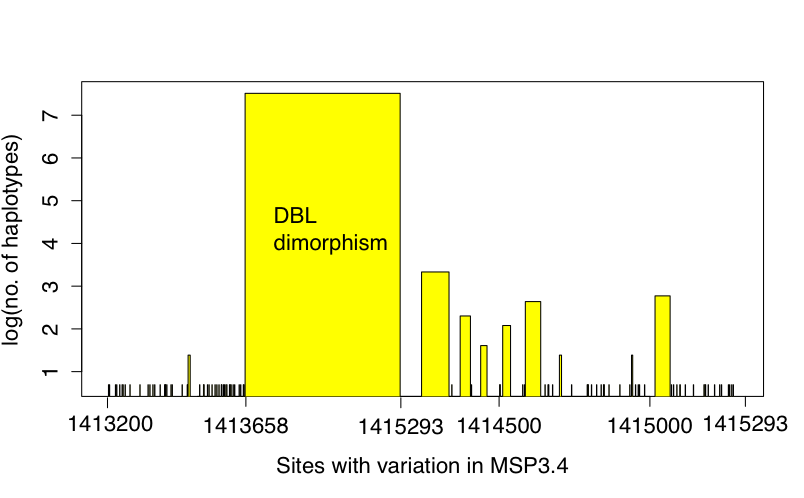
\includegraphics[height=5cm]{PRG.png}
\caption{Histogram of number of alleles at each site in MSP3.4 plotted above the chromosome coordinate.)}
\label{fig:example}
\end{figure}

\textit{P. falciparum} is a haploid malaria parasite that undergoes recombination when inside a mosquito. It has an unusually repetitive genome that contains more indels than SNPs \cite{miles}. There are several regions that present challenges to mapping because samples often diverge strongly from the reference. Should say something about vaccine targets here? For example, the merozoite surface protein gene MSP3.4 is known to have two highly diverged lineages at high frequencies in multiple populations from across the world.  The lineages differ by around 1 SNP every 3 bases over a 500bp region (the DBL domain) of the gene.




We constructed a catalog of MSP3.4 variation from Cortex \cite{iqbal} and GATK \cite{depristo} variant calls from 700 \textit{P. falciparum} samples from the Ghana, Laos and Cambodia, and built a PRG just for that chromosome. We aligned Illumina 100bp reads from a well-studied sample that was not used in graph construction (named 7G8) to the PRG using backward search (exact matching), and collected counts on the number of reads supporting each allele. We used a simple ``heaviest path" method similar to that outlined by Valenzuela et al \cite{valen} (NOT sure this is right, they are doing something a bit different) to choose the path through the graph which best supported the data. This was our graph-inferred personalised reference for this sample. We then mapped the reads (using bwa\_mem \cite{hengli}) to the inferred genome. As can be seen in Figure 6, this gives dramatically better pileup results over the MSP3.4 gene. For validation, we compared our graph-inferred version of the gene with a high-quality assembly from PacBio sequencing (87X coverage?), which confirmed our results. 


\begin{figure}[!tbp]
  \centering
  \begin{minipage}[b]{0.4\textwidth}
    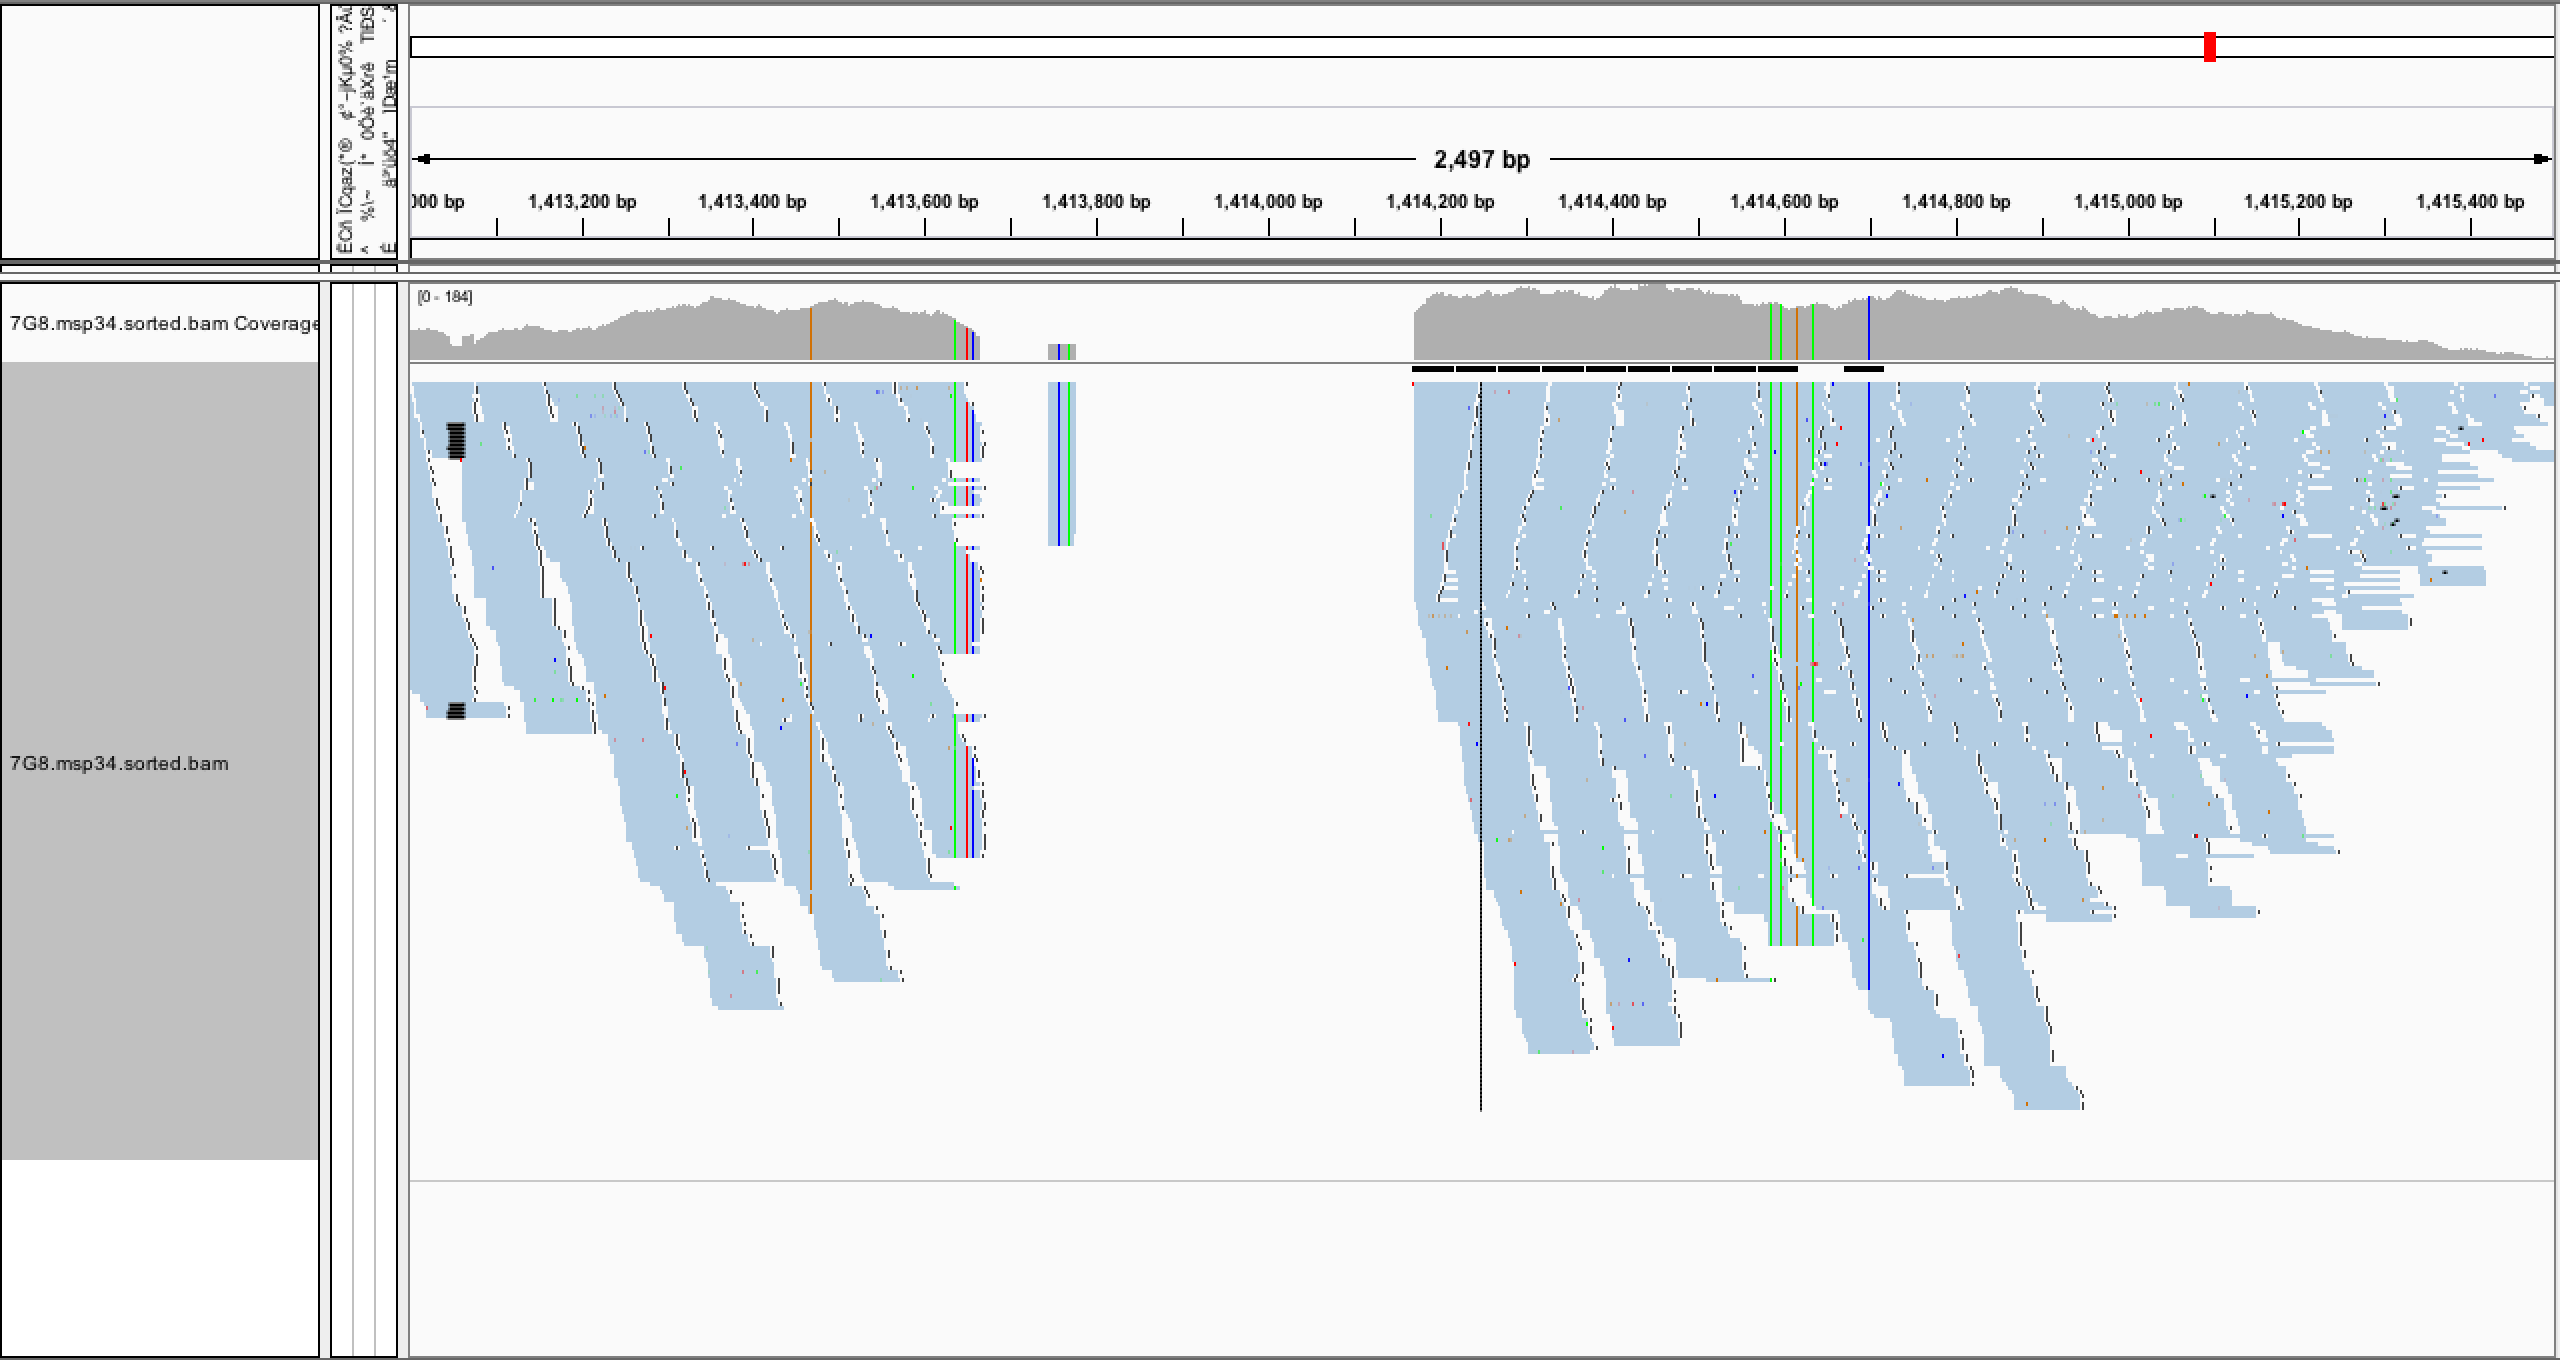
\includegraphics[width=\textwidth]{7G8_to_3D7_pileup.png}
    \caption{Mapping reads from sample 7G8 to \textit{P. falciparum} 3D7 reference genome results in a gap.}
  \end{minipage}
  \hfill
  \begin{minipage}[b]{0.45\textwidth}
    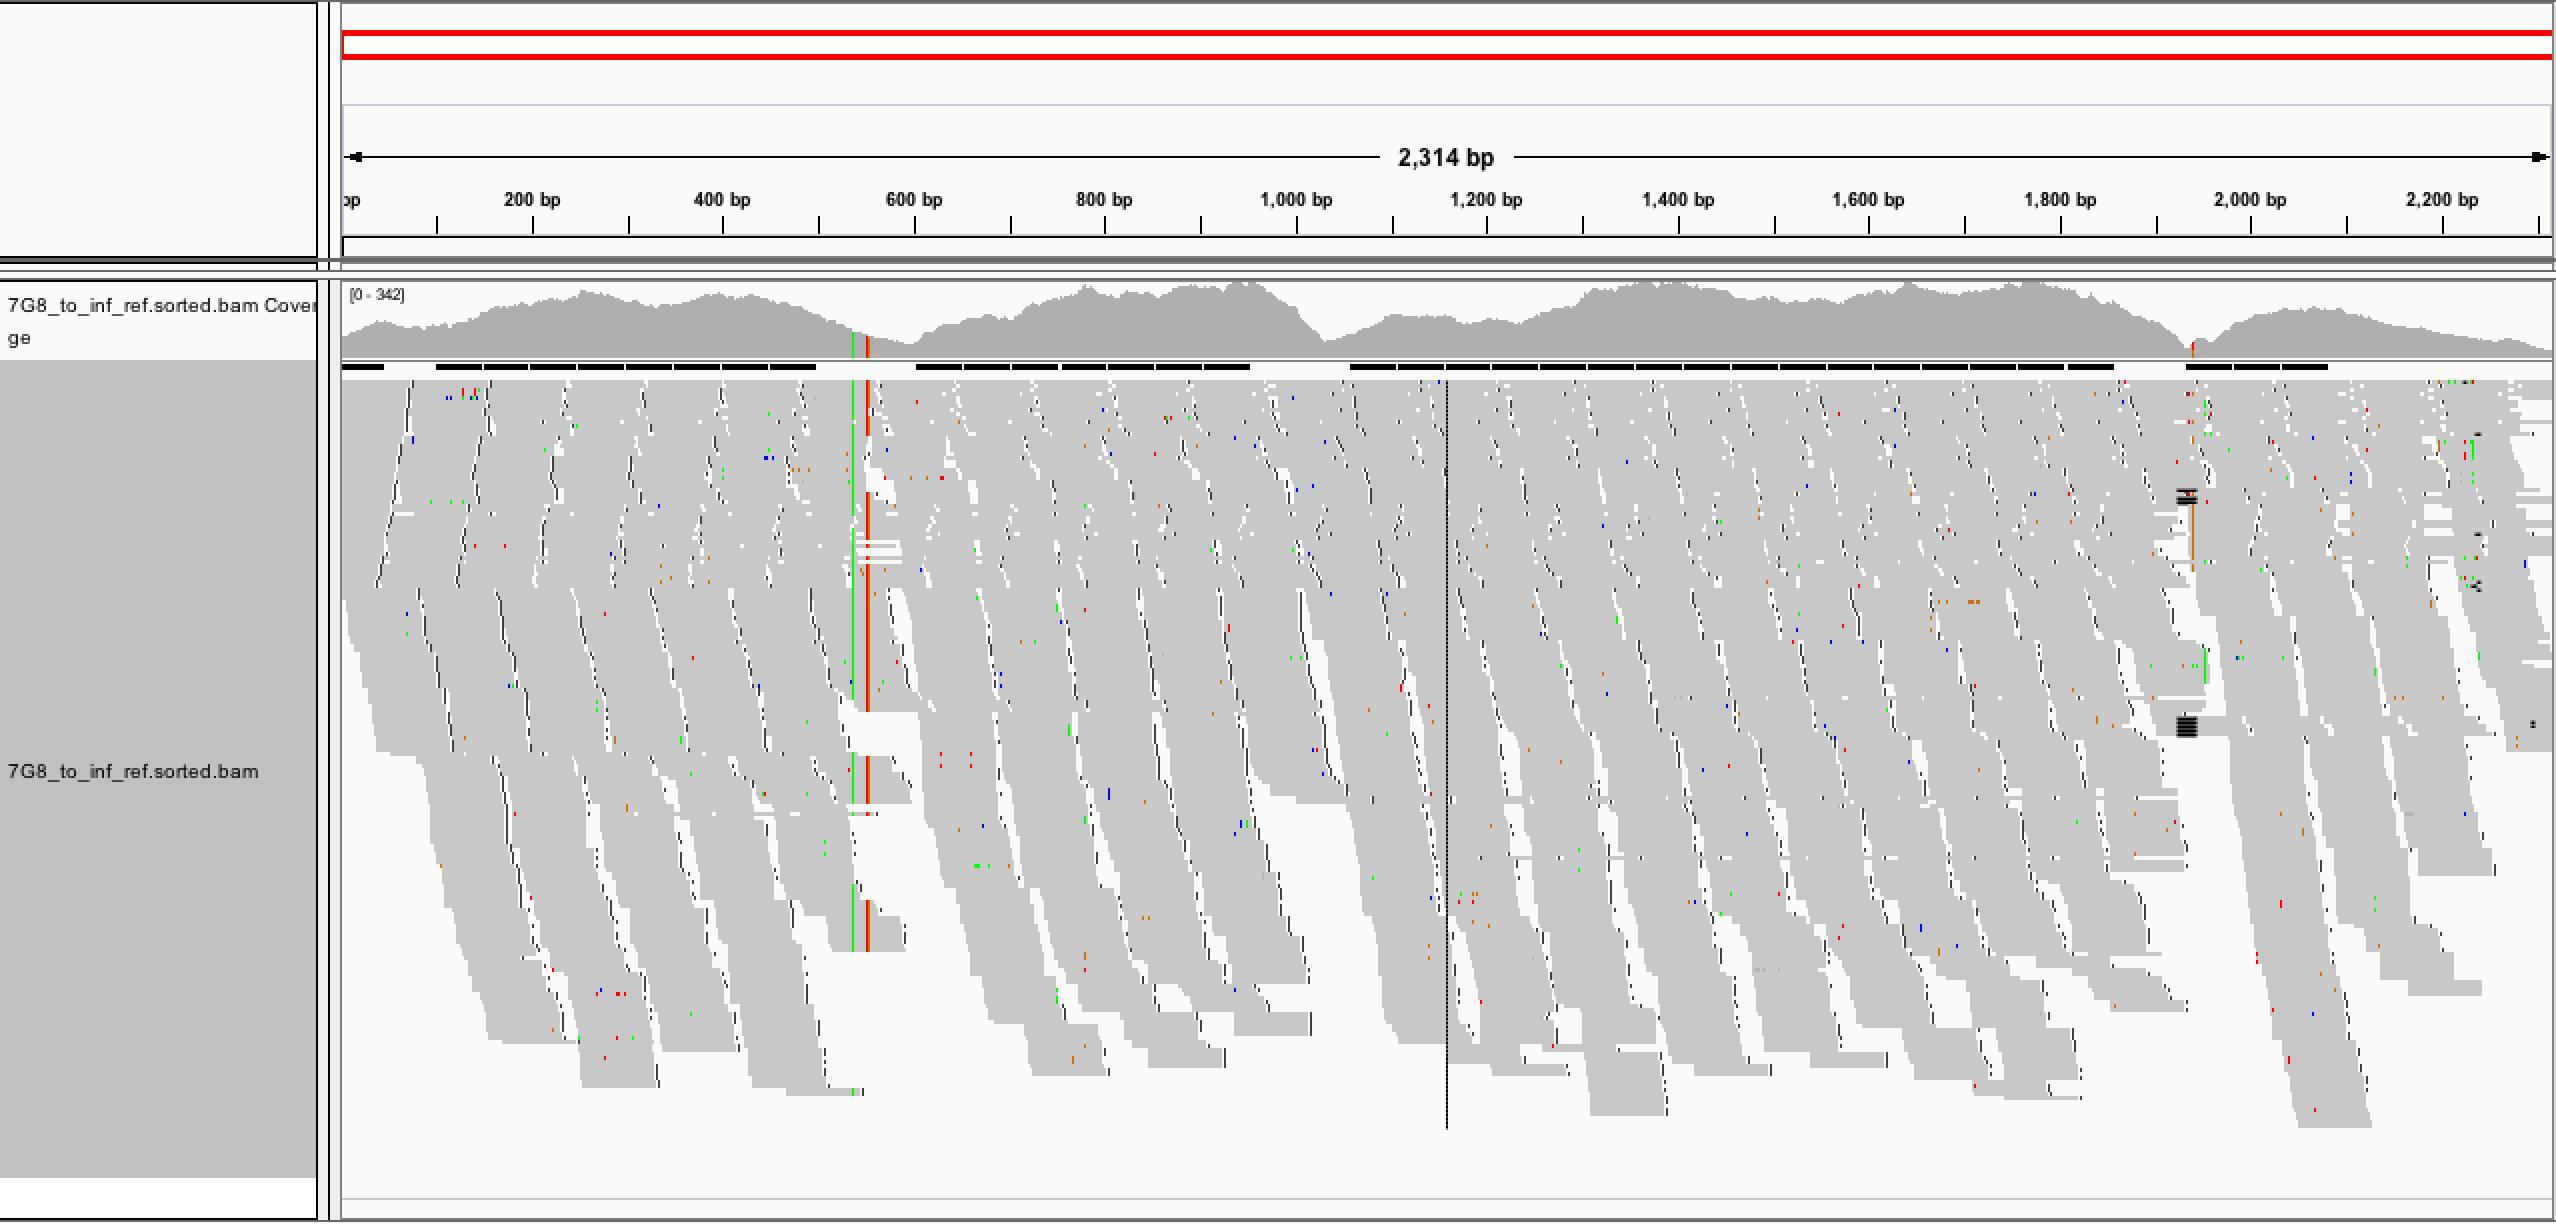
\includegraphics[width=\textwidth]{7G8_to_inf_ref_pileup.png}
    \caption{Mapping reads from sample 7G8 to our vBWT-inferred genome removes the gap, leaving isolated variants easy to detect with standard methods }
  \end{minipage}
\end{figure}






\subsection{Further performance comments}
One  consequence of our approach, shared with bwbble, is that a single pattern can match multiple intervals in the BWT. Thus for mapping we store a list of intervals, along with which sites and alleles are crossed. Our current implementation of this is naive (using C++ std::unordered\_map). We also store an integer array (mask) allowing us to determine if a position in the PRG is in a site, and if so, which allele - again naively encoded (in std::vector). For the human genome example these cost us around 12GB of RAM. This sparse  array, which contains a zero at every non-variable site in the chromosome,  could be stored much more compactly.

This encoding results in an alphabet of size $4+2n$ where $n$ is the number of variant sites. We used the wavelet tree to mitigate this cost from O(n) to O(log(n)), but to get an estimate of how this impacts performance in practise, we measure speed of exact matching of simulated perfect reads from \textit{P. falciparum} chromosome 10 with only MSP3.4 variation inserted. To avoid unnecessarily repeatedly shrinking the same BWT intervals, we store  in a hash the  BWT intervals corresponding to all 9-mers in the PRG. This results in read-matching at a rate of 277/second.



Finally, there is one performance improvement which we have yet to implement - precalculating and storing an array of ranks at marker positions across the BWT - just as in a standard FM-index. This is not normally done for large alphabet wavelet-tree-based suffix arrays, but we can ignore the numeric characters, and store only for A,C,G,T. 

\section{Discussion}
By extending the alphabet and placing positional markers, we are able to ensure that alternate alleles sort together in the BWT matrix, allowing mapping across sites and recombination. In fact, we could encode quite general graph structures in this manner, but for simplicity we imposed a constraint on graph construction, and did not allow nesting of sites. For haploids, the idea of systematically choosing a closer reference, and then using the standard tools is easily communicated and can be directly integrated into standard analyses. Secondly, for other ploidies, our implementation readily lends itself to collecting phase-informative read-data, running an HMM, and finally MEM-based graph alignment. We have made a choice to encode genetic variation as a Directed Acyclic Graph - thus inversions or rearrangements must be encoded as explicit alternate alleles. Our choice was deliberate - we are aiming for a more limited model, but avoiding heuristics in the details of the graph construction, especially in regions of high diversity. 






\subsubsection{Software}
We have implemented the vBWT twice. First as a simple prototype, which provided the results on \textit{P. falciparum} above. Secondly,  a more careful implementation that provided all other results, and which is available here: http://github.com/iqbal-lab/gramtools. We make the prototype available here purely for sake of reproducibility URL, but all future development (and maintenance) is on the second implementation.



\subsubsection*{Acknowledgments.} We would like to thank Jerome Kelleher, Heng Li, Rayan Chikhi and Jouni Siren for discussions, and Lin Huang and Victoria Popic for help running bwbble. Above all we would like to thank Simon Gog and the SDSL developers for providing a valuable and well-maintained resource. <FUNDING>



\begin{thebibliography}{4}

\bibitem{valen} Valenzuela, D., Valimaki, N., Pitkanen, E., Makinen, V. On enhancing variation detection through pan-genome indexing. Biorxiv. http://dx.doi.org/10.1101/021444

\bibitem{bwt} Burrows, M., Wheeler, D.J. :A block sorting lossless data compression algorithm. Digital Equipment Corporation, Tech. Rep. 124, 1994. Available: http://www.hpl.hp.com/ techreports/Compaq-DEC/SRC-RR-124.html

\bibitem{bwa} Li, H., Durbin, R.: Fast and accurate short read alignment with Burrows?Wheeler transform. Bioinformatics 25 (14): 1754-1760 (2009)

\bibitem{bowtie} Langmead, B., Salzberg, S.: Fast gapped-read alignment with Bowtie 2. Nature Methods. Mar 4;9(4):357-9 (2012)

\bibitem{reinert} Reinert, K., Langmead, B., Weese, D., et al: Alignment of Next-Generation Sequencing Reads. Annu Rev Genomics Hum Genet. 2015;16:133-51

\bibitem{1000g} The 1000 Genomes Project Consortium: A global reference for human genetic variation. Nature 526, 68?74

\bibitem{arabi} Ossowski, S., Schneeberger, K., Clark, R.M., et al. Sequencing of natural strains of Arabidopsis thaliana with short reads. Genome Research 18, 2024-2033 (2008)

\bibitem{pombe} Jeffares, D.C., Rallis, C., Rieux, A., et al. The genomic and phenotypic diversity of Schizosaccharomyces pombe. Nature Genetics 47, 235?241 (2015)

\bibitem{dilthey} Dilthey, A., Cox, C., Iqbal, Z., et al: Improved genome inference in the MHC using a population reference graph. Nature Genetics 47, 682?688 (2015)

\bibitem{korbinian} Schneeberger, K.,Hagmann, J., Ossowski, S.,  et al. Simultaneous alignment of short reads against multiple genomes. Genome Biol. 10, R98 (2009).

\bibitem{siren1} Siren, J., Valimaki, N., Makinen, V. Indexing Graphs for Path Queries with Applications in Genome Research. IEEE/ACM Trans Comput Biol Bioinform. 2014 Mar-Apr;11(2):375-88

\bibitem{huang} Huang, L., Popic, V., Batzoglou, S. Short read alignment with populations of genomes. Bioinformatics. Jul 1;29(13):i361-70 (2013)

\bibitem{siren2} Siren, J. Indexing Variation Graphs. 	arXiv:1604.06605 

\bibitem{na} Na, J.C., Crochemore, M., Park, H.,  et al: Suffix tree of alignment: an efficient index for similar data. Combinatorial Algorithms ? Revised Selected Papers of the 24th International Workshop, IWOCA 2013, Rouen, France, July 10?12, 2013 (2013), pp. 337?348

\bibitem{miles} Miles, A., Iqbal, Z., Vauterin, P., et al .: Genome variation and meiotic recombination in Plasmodium falciparum: insights from deep sequencing of genetic crosses Biorxiv. http://dx.doi.org/10.1101/024182 (2015)

\bibitem{iqbal} Iqbal, Z., Caccamo, M. Turner, I.,  et al: De novo assembly and genotyping of variants using colored de Bruijn graphs. Nature Genetics  44, 226?232 (2012)

\bibitem{depristo} DePristo, M., Banks, E., Poplin, R.E., et al: A framework for variation discovery and genotyping using next-generation DNA sequencing data. Nature Genetics 43(5): 491?498 (2011)

\bibitem{hengli} Li, H. Aligning sequence reads, clone sequences and assembly contigs with BWA-MEM. 	arXiv:1303.3997


\end{thebibliography}


\section{Checklist of Items to be Sent to Volume Editors}
Here is a checklist of everything the volume editor requires from you:


\begin{itemize}
\settowidth{\leftmargin}{{\Large$\square$}}\advance\leftmargin\labelsep
\itemsep8pt\relax
\renewcommand\labelitemi{{\lower1.5pt\hbox{\Large$\square$}}}

\item The final \LaTeX{} source files
\item A final PDF file
\item A copyright form, signed by one author on behalf of all of the
authors of the paper.
\item A readme giving the name and email address of the
corresponding author.
\end{itemize}
\end{document}
